\documentclass[a4paper]{book}
\usepackage[utf8]{inputenc}
\usepackage{graphicx}
\usepackage[T1]{fontenc} 
\usepackage[spanish]{babel}
\usepackage{titlesec}
\usepackage{geometry}
\usepackage{float}
\usepackage{verbatim}
\usepackage{booktabs}
\usepackage{colortbl}
\usepackage[table]{xcolor}
\usepackage{array}
\usepackage{tabularx}
\usepackage{hyperref}
\usepackage{fancyhdr}
\usepackage{lipsum}


\hypersetup{
    colorlinks=true,
    linkcolor=blue,
    urlcolor=blue,
    filecolor=magenta,      
    citecolor=blue,
    pdftitle={SafeSight - Proyecto Argos},
    pdfauthor={Edwin Benito Castillo Hernández, David de Jesús Hernández Hernández, Alfonso Oropeza Sangabriel, Erick Rivas Esquivel},
    %bookmarks=true,
    pdfpagemode=FullScreen,
}

\titleformat{\chapter}[display]
  {\normalfont\huge\bfseries}{\chaptertitlename\ \thechapter}{20pt}{\Huge}
\titlespacing*{\chapter}{0pt}{-30pt}{20pt}

\let\cleardoublepage\clearpage

\setcounter{secnumdepth}{3}
\setcounter{tocdepth}{3}

\begin{document}


\begin{titlepage}
    \centering

    
\includegraphics[width=0.3\textwidth]{logo_upp.jpg}\par

    \vspace{1cm}
    {\Huge\bfseries Universidad Politécnica de Pachuca\par}
    \vspace{2cm}

    {\Large\bfseries SafeSight\par}
    \vspace{1cm}

    {\Huge\bfseries Proyecto Argos\par}
    \vspace{1.5cm}

    {\Large Ingeniería en Tecnologías de la Información e Innovación Digital\par}
    \vspace{1cm}

    {\large\bfseries Integrantes:\par}
    \vspace{0.5cm}
    {\large Castillo Hernández Edwin Benito -- 2431124902\par}
    {\large Hernández Hernández David de Jesús -- 2431124979\par}
    {\large Oropeza Sangabriel Alfonso -- 2431124918\par}
    {\large Rivas Esquivel Erick -- 2431124895\par}
    \vspace{0.5cm}

    {\large\bfseries PROYECTO INTEGRADOR I\par}
    {\large\bfseries TÓPICOS DE CALIDAD PARA EL DISEÑO DE SOFTWARE\par}
    {\large\bfseries DESARROLLO DEL PENSAMIENTO Y TOMA DE DECISIONES\par}
    
    \vspace{1cm}

    {\large Mayo-agosto 2025\par}
    \vfill

    \thispagestyle{empty}
\end{titlepage}







\frontmatter
\tableofcontents

\mainmatter
\clearpage
\chapter{Perfil de Proyecto}

\section{Identificación y Análisis del Problema}




En la Universidad Politécnica de Pachuca, el registro de entrada y asistencia provoca saturación en los accesos debido a procesos manuales y falta de tecnología adecuada. Esta situación genera retrasos para los alumnos, dificulta el inicio puntual de las clases y complica el registro para los padres, afectando la convivencia y el orden institucional.

La acumulación de personas en los puntos de acceso impacta la dinámica diaria y la experiencia de la comunidad universitaria.


%\clearpage
\section{Objetivos del Proyecto}

\subsection{Objetivo General}


Establecer un sistema de control eficiente de usuarios en la Universidad Politécnica de Pachuca con el fin de garantizar la seguridad, el registro automatizado de accesos y la trazabilidad de la asistencia escolar.

\subsection{Objetivos Específicos}

\begin{itemize}
    \item Implementar un mecanismo de reconocimiento facial que registre la entrada del alumnado a la institución educativa.
    \item Proporcionar a los docentes una herramienta digital para verificar la asistencia de los estudiantes a sus respectivas clases.
    \item Desarrollar una plataforma en línea que permita a los padres de familia consultar en tiempo real la asistencia de sus hijos tanto al plantel como a sus clases programadas.
    \item Restringir el acceso a personas no autorizadas, reforzando la seguridad del entorno escolar mediante validaciones tecnológicas.
\end{itemize}

\clearpage
\section{Necesidades Tecnológicas}

El sistema Argos requiere infraestructura tecnológica adecuada: dispositivos biométricos, redes confiables, servidores y plataformas digitales. Estos recursos permiten automatizar procesos y proteger la información.

La siguiente imagen muestra el esquema básico de la solución tecnológica propuesta.
\subsection{Mapa Mental}

\begin{figure}[H]
    \centering
    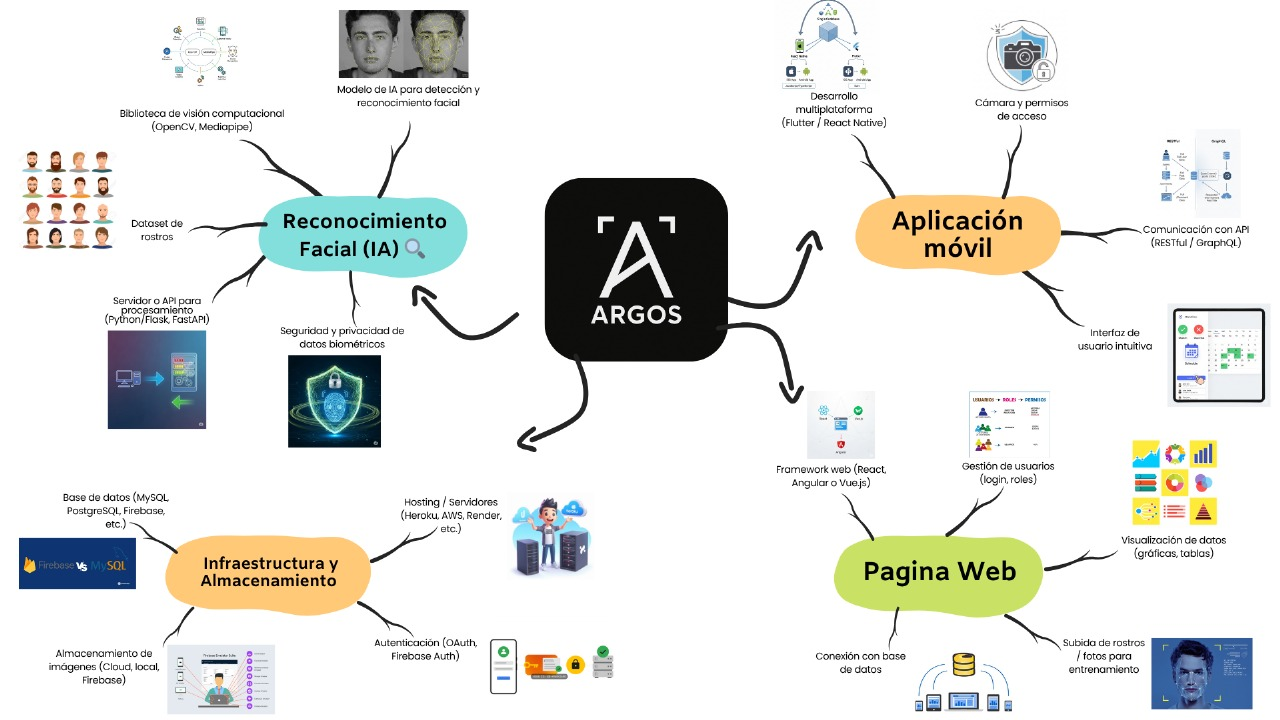
\includegraphics[width=1.0\textwidth]{./Media/mapaArgos.jpg}
    \caption{Mapa general de la infraestructura tecnológica propuesta para Argos}
    \label{fig:infraestructura}
\end{figure}

\clearpage
\section{Evaluación de Condiciones y Necesidades del Proyecto}

\subsection{Técnicas para identificar problemas}

La identificación de problemas es un paso fundamental en el desarrollo de un proyecto, esto permite comprender las necesidades 
reales del contexto, los usuarios y las organizaciones involucradas. A continuación, se describen las técnicas básicas 
utilizadas en esta etapa: Estas técnicas fueron seleccionadas considerando la diversidad de actores involucrados 
(alumnos, personal administrativo, padres de familia, docentes) y la complejidad del sistema propuesto.

\subsubsection*{Análisis de Cuestionarios y Entrevistas}
Durante el mes de junio se aplicaron encuestas y entrevistas presenciales en las instalaciones de la
 Universidad Politécnica de Pachuca, principalmente en horarios de entrada y salida escolar. El objetivo de esta técnica 
 fue identificar necesidades, dificultades y expectativas de los usuarios clave respecto al sistema propuesto. 
 Su utilidad radica en que permitió obtener información directa y variada de alumnos, docentes y personal administrativo, 
 facilitando la detección de problemas y oportunidades de mejora.

\subsubsection*{Observación Directa}
Esta técnica se llevó a cabo durante junio en los accesos principales de la institución, en los horarios de mayor afluencia. 
El objetivo fue analizar el comportamiento real de los usuarios y los procesos actuales de registro de entrada.
 La observación directa resultó útil para detectar problemas no expresados verbalmente y observar el flujo real de personas y 
 los tiempos de espera.

\subsubsection*{Consulta con Expertos}
Durante el mes de junio se realizaron reuniones presenciales y virtuales con especialistas en tecnologías de la información 
y gestión escolar. El objetivo fue validar la viabilidad técnica y operativa de la solución propuesta. 
Esta técnica fue útil porque aportó recomendaciones sobre integración tecnológica, seguridad y
 mejores prácticas, anticipando posibles retos y permitiendo ajustar el diseño conceptual del sistema.





% Para que las subsubsecciones aparezcan numeradas y en el índice
\setcounter{secnumdepth}{3}
\setcounter{tocdepth}{3}


\clearpage

\subsection{Método Delphi}

El método \textbf{Delphi} es una técnica de pronóstico que busca el consenso de un grupo de expertos. Se basa en rondas de cuestionarios anónimos, donde la retroalimentación gradual converge hacia un acuerdo. Para el desarrollo del proyecto \textbf{Argos}, la empresa \textbf{SafeSight} aplicó este método para evaluar y refinar la propuesta de sistema de control de acceso escolar con reconocimiento facial, asegurando una solución robusta y adaptada a la comunidad educativa.

\begin{figure}[H]
    \centering
    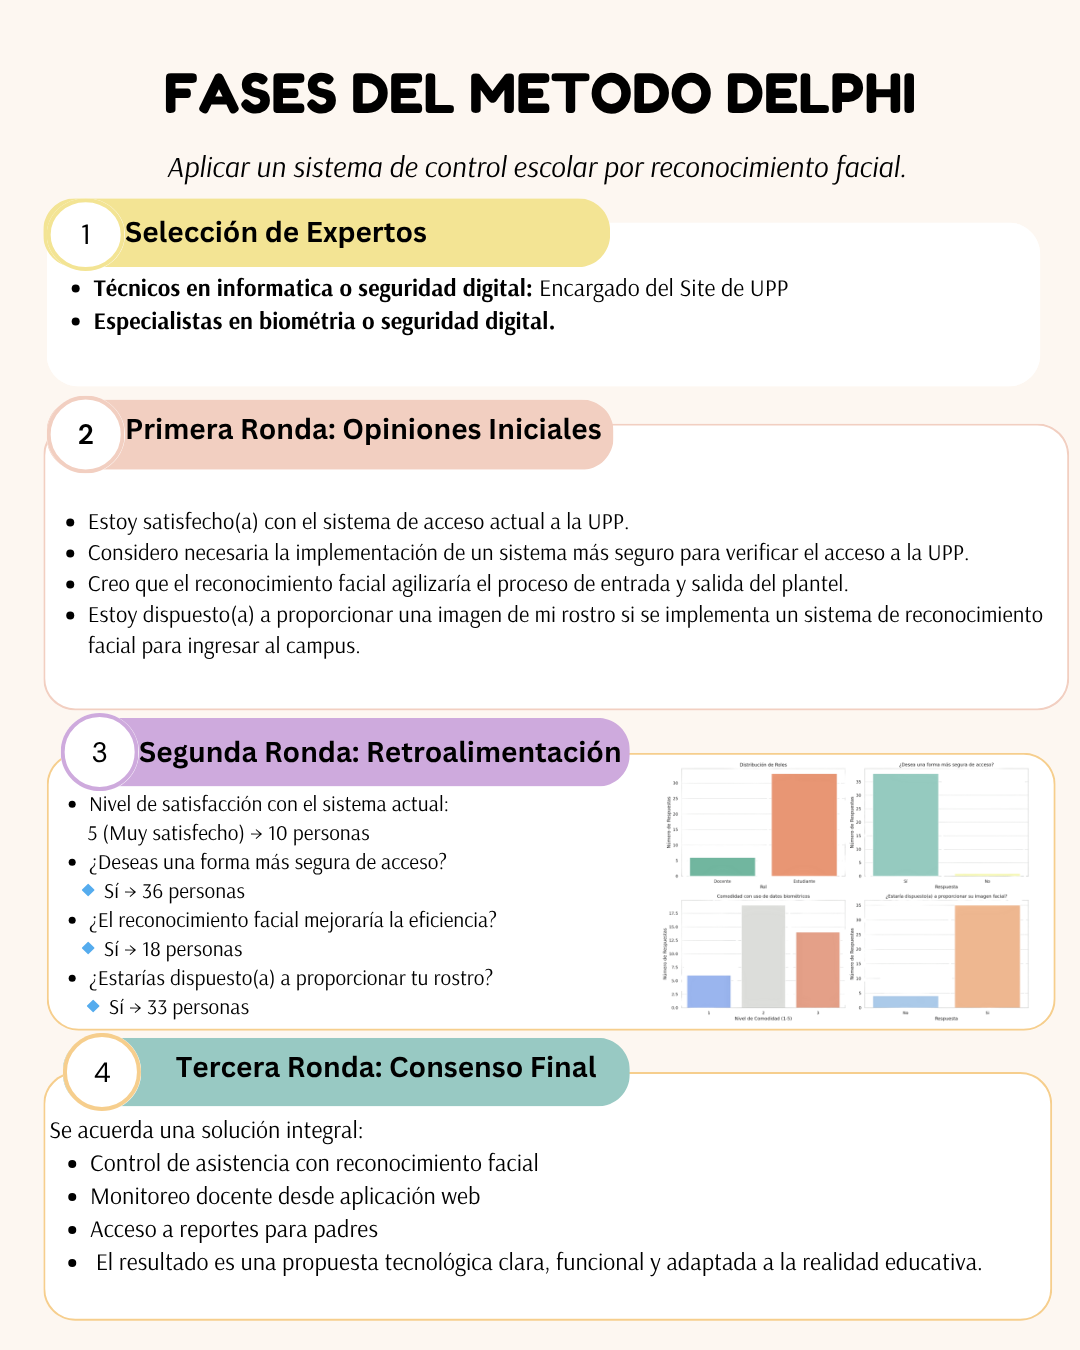
\includegraphics[width=0.85\textwidth]{./Media/Delphi.png}
    \caption{Ejemplo de aplicación del Método Delphi por SafeSight para el proyecto Argos}
    \label{fig:delphi}
\end{figure}

\clearpage
\section{Visión del Proyecto}

El proyecto Argos busca modernizar el acceso y la asistencia escolar en la Universidad Politécnica de Pachuca con un sistema automatizado, seguro y eficiente. A corto plazo, reducirá los tiempos de acceso y errores en el registro; a mediano, mejorará la comunicación y el monitoreo de asistencia; y a largo plazo, consolidará un entorno escolar innovador y confiable. Argos fortalecerá la confianza, la puntualidad y la toma de decisiones, y servirá como modelo para otras instituciones educativas.

Además, Argos impulsará el desarrollo de competencias digitales en la comunidad escolar y facilitará la adaptación a nuevas tecnologías, contribuyendo al crecimiento institucional y al bienestar de todos los usuarios involucrados.


%\clearpage
\section{Alcance del Proyecto}


El presente proyecto se enfoca en el análisis, planeación, diseño y pruebas de usabilidad de una solución para optimizar el control de acceso y la gestión de la asistencia en entornos educativos, tomando como referencia la Universidad Politécnica de Pachuca. La implementación de esta solución se plantea como un proyecto a largo plazo, con la intención de abordar las necesidades actuales y futuras de la institución educativa.


El proyecto no contempla el desarrollo ni la implementación de sistemas de seguridad física, como cámaras de vigilancia o alarmas, ni la integración con sistemas externos de control de acceso que no sean los mencionados. Asimismo, por el momento no contempla el reconocimiento facial como mecanismo de identificación.



%\clearpage
\section{Público Objetivo}


El público objetivo del proyecto está centrado en la Universidad Politécnica de Pachuca, e incluye a:

\begin{itemize}
\item Alumnos (usuarios finales)
\item Docentes
\item Visitantes
\item Personal administrativo (Secretaría, Control Escolar)
\item Dirección escolar / Rectoría
\item Proveedores de servicios
\item Personal de seguridad escolar
\item Padres de familia (beneficiarios indirectos)
\end{itemize}

\clearpage
\section{Recursos Disponibles}


Para la correcta ejecución y desarrollo del proyecto, se identificaron y organizaron los recursos disponibles en las siguientes categorías: humanos, materiales, tecnológicos y servicios. A continuación, se presentan las tablas correspondientes a cada tipo de recurso:

\subsection{Recursos Humanos}

% Recursos Humanos
\begin{table}[h!]
\centering
\footnotesize
\setlength{\tabcolsep}{3.5pt}
\renewcommand{\arraystretch}{0.98}
\begin{tabular}{|l|c|}
\hline
	extbf{Recurso Humano} & \textbf{Costo mensual (MXN)} \\
\hline
Líder de Proyecto Jr & \$25,000 \\
Analista Jr & \$20,000 \\
Diseñador UI/UX Jr & \$20,000 \\
Desarrollador de IA Jr & \$40,000 \\
Desarrollador Mobile Jr & \$36,000 \\
Desarrollador Backend Jr & \$35,000 \\
Desarrollador Frontend Jr & \$33,000 \\
QA Jr & \$18,000 \\
Administrador de Base de Datos Jr & \$22,000 \\
Especialista en Seguridad Jr & \$25,000 \\
Consultor en Reconocimiento Facial Jr & \$28,000 \\
\hline
	extbf{Total Recursos Humanos} & \textbf{\$302,000} \\
\hline
\end{tabular}
\caption{Recursos humanos y costos mensuales estimados}
\end{table}

\subsection{Recursos Materiales y Tecnológicos}

% Recursos Materiales y Tecnológicos
\begin{table}[h!]
\centering
\footnotesize
\setlength{\tabcolsep}{3.5pt}
\renewcommand{\arraystretch}{0.98}
\begin{tabular}{|l|c|}
\hline
\textbf{Recurso Material/Tecnológico} & \textbf{Costo mensual (MXN)} \\
\hline
Cámaras de reconocimiento facial (3 unidades) & \$3,000 \\
Servidores en la nube & \$2,500 \\
Licencias de software & \$1,200 \\
Internet y servicios de red & \$1,000 \\
Material de oficina y papelería & \$500 \\
\hline
\textbf{Total Material/Tecnológico} & \textbf{\$8,200} \\
\hline
\end{tabular}
\caption{Recursos materiales y tecnológicos y costos mensuales estimados}
\end{table}

\subsection{Servicios y Capacitación}

% Servicios y capacitación
\begin{table}[h!]
\centering
\footnotesize
\setlength{\tabcolsep}{3.5pt}
\renewcommand{\arraystretch}{0.98}
\begin{tabular}{|l|c|}
\hline
\textbf{Servicio/Capacitación} & \textbf{Costo mensual (MXN)} \\
\hline
Capacitación y talleres & \$2,000 \\
Mantenimiento de equipos & \$1,500 \\
Soporte externo & \$1,800 \\
\hline
\textbf{Total Servicios/Capacitación} & \textbf{\$5,300} \\
\hline
\end{tabular}
\caption{Servicios y capacitación y costos mensuales estimados}
\end{table}

% Total general
\vspace{0.5cm}
	{Costo total mensual estimado:} \$315,500 MXN

%%==========================================================================================%

\clearpage
\chapter{Planeación del Proyecto}




\section{Roles Principales}
\begingroup
\small

\subsection*{1. Líder de Proyecto (Project Manager)}
\textbf{Rivas Esquivel Erick}\\
Responsabilidades:
\begin{itemize}
    \item Coordinar al equipo y dar seguimiento al cronograma.
    \item Facilitar la comunicación entre los integrantes.
    \item Controlar entregables, tiempos y cumplimiento de objetivos.
    \item Convocar reuniones y documentar acuerdos.
\end{itemize}

\subsection*{2. Analista de Requerimientos}
\textbf{David de Jesús Hernández Hernández}\\
Responsabilidades:
\begin{itemize}
    \item Investigar y documentar las necesidades del cliente/usuario.
    \item Redactar documentos como el de visión y alcance.
    \item Elaborar casos de uso, historias de usuario o requisitos funcionales y no funcionales.
    \item Validar requerimientos con los stakeholders.
\end{itemize}

\subsection*{3. Diseñador de Interfaces de Usuario (UI/UX)}
\textbf{Oropeza Sangabriel Alfonso}\\
Responsabilidades:
\begin{itemize}
    \item Crear wireframes, prototipos y mockups.
    \item Aplicar principios de usabilidad y diseño centrado en el usuario.
    \item Coordinar pruebas de usabilidad.
    \item Documentar la matriz de tareas y contenido de usuario.
\end{itemize}

\subsection*{4. Encargado de Calidad}
\textbf{Castillo Hernández Edwin Benito}\\
Responsabilidades:
\endgroup
\begin{itemize}
    \item Definir y aplicar estándares de calidad del producto y del proceso.
    \item Verificar que cada entregable cumpla los criterios establecidos.
    \item Realizar auditorías internas del proyecto.
    \item Coordinar retroalimentaciones para mejora continua.
\end{itemize}


\clearpage
\section{Diagrama de Gantt del Proyecto Argos}

La planeación del proyecto Argos se estructura en tareas clave distribuidas a lo largo de once semanas, permitiendo una gestión ordenada y eficiente de los recursos y actividades.

\begin{table}[htbp]
  \centering
  \caption{Correspondencia de semanas, meses y fechas aproximadas}
  \rowcolors{2}{gray!10}{white}
  \begin{tabular}{ccc}
    \toprule
    \rowcolor{gray!30}
    \textbf{Semana} & \textbf{Mes} & \textbf{Fecha aproximada} \\
    \midrule
    S1  & Junio  & 3--7~junio \\
    S2  & Junio  & 10--14~junio \\
    S3  & Junio  & 17--21~junio \\
    S4  & Junio  & 24--28~junio \\
    S5  & Julio  & 1--5~julio \\
    S6  & Julio  & 8--12~julio \\
    S7  & Julio  & 15--19~julio \\
    S8  & Julio  & 22--26~julio \\
    S9  & Julio  & 29~julio--2~agosto \\
    S10 & Agosto & 5--9~agosto \\
    S11 & Agosto & 12--16~agosto \\
    \bottomrule
  \end{tabular}
  \label{tab:semanas_meses_fechas}
\end{table}


\begin{table}[htbp]
  \centering
  \caption{Planeación de actividades del proyecto Argos por semana}
  \rowcolors{2}{gray!10}{white}
  \begin{tabular}{lccccccccccc}
    \toprule
    \rowcolor{gray!30}
    \textbf{Actividad} & \textbf{S1} & \textbf{S2} & \textbf{S3} & \textbf{S4} & \textbf{S5} & \textbf{S6} & \textbf{S7} & \textbf{S8} & \textbf{S9} & \textbf{S10} & \textbf{S11} \\
    \midrule
    Análisis del Problema & \cellcolor{green!30}$\bullet$ & \cellcolor{green!30}$\bullet$ & \cellcolor{green!30}$\bullet$ & \cellcolor{green!30}$\bullet$ & \cellcolor{green!30}$\bullet$ &  &  &  &  &  &  \\
    Recolección de Requerimientos &  &  & \cellcolor{blue!20}$\bullet$ & \cellcolor{blue!20}$\bullet$ & \cellcolor{blue!20}$\bullet$  & \cellcolor{blue!20}$\bullet$  &  &  &  &  &  \\
    Diseño de Interfaz de Usuario &  & \cellcolor{orange!30}$\bullet$ & \cellcolor{orange!30}$\bullet$ & \cellcolor{orange!30}$\bullet$ & \cellcolor{orange!30}$\bullet$ & \cellcolor{orange!30}$\bullet$ & \cellcolor{orange!30}$\bullet$ &  &  &  &  \\
    Revisión de Documentación &  &  &  &  &  & \cellcolor{purple!20}$\bullet$ & \cellcolor{purple!20}$\bullet$ &  &  &  &  \\
    Pruebas Usabilidad &  &  &  &  &  &  &  &  & \cellcolor{cyan!20}$\bullet$ & \cellcolor{cyan!20}$\bullet$ &  \\
    Validación de entregables &  &  &  &  &  &  &  & \cellcolor{red!20}$\bullet$ & \cellcolor{red!20}$\bullet$ &  &  \\
    Presentación del Proyecto (20 de Agosto) &  &  &  &  &  &  &  &  &  & \cellcolor{gray!60}$\bullet$ & \cellcolor{gray!60}$\bullet$ \\
    \bottomrule
  \end{tabular}
  \label{tab:planeacion_argos}
\end{table}

\clearpage
\section{Ruta Crítica del Proyecto}

\subsection{Tabla de Actividades del Proyecto}
Esta tabla desglosa las actividades principales del proyecto, sus duraciones estimadas en días y las dependencias entre ellas. Se considera que cada semana equivale a 5 días hábiles. La suma de las duraciones es de 100 días hábiles (esfuerzo total), pero la duración real del proyecto, determinada por la ruta crítica y el diagrama de Gantt, es de 10 semanas hábiles (50 días), distribuidas a lo largo de 11 semanas calendario. Las dependencias indican qué actividades deben completarse antes de que otra pueda comenzar.

\begin{table}[htbp]
  \centering
  \caption{Tabla de Actividades del Proyecto}
  \renewcommand{\arraystretch}{1.3}
  \setlength{\tabcolsep}{7pt}
  \rowcolors{2}{gray!10}{white}
  \begin{tabularx}{\linewidth}{>{\centering\arraybackslash}p{1.2cm} X >{\centering\arraybackslash}p{2.2cm} >{\centering\arraybackslash}p{2.2cm}}
    \toprule
    \rowcolor{gray!30} \textbf{ID} & \textbf{Actividad} & \textbf{Duración (Días)} & \textbf{Predecesoras} \\
    \midrule
  A & Análisis del Problema & 20 & --- \\
    B & Recolección de Requerimientos & 20 & A \\
    C & Diseño de Interfaz de Usuario & 30 & B \\
    D & Revisión de Documentación & 5 & C \\
    E & Pruebas Usabilidad & 10 & D \\
    F & Validación de Entregables & 10 & D \\
    G & Presentación del Proyecto & 5 & E, F \\
    \bottomrule
  \end{tabularx}
\end{table}
\vspace{0.7em}
\noindent\textbf{Nota:} Aunque la suma de las duraciones de las actividades es 100 días hábiles, el proyecto se ejecuta realmente en 10 semanas hábiles (50 días), con un horizonte de 11 semanas calendario, debido al paralelismo entre actividades.

\clearpage
\subsection{Cálculos de ES y EF (Paso Hacia Adelante)}

El "Paso Hacia Adelante" (Forward Pass) se utiliza para determinar la Fecha de Inicio Temprana (ES - Early Start) y la Fecha de Finalización Temprana (EF - Early Finish) para cada actividad, ahora en días hábiles (1 semana = 5 días).

\begin{itemize}
    \item \textbf{ES (Fecha de Inicio Temprana):} La fecha más temprana en que una actividad puede comenzar, asumiendo que todas sus predecesoras se han completado.
    \item \textbf{EF (Fecha de Finalización Temprana):} La fecha más temprana en que una actividad puede terminar. Se calcula como $EF = ES + Duración$.
\end{itemize}

\begin{table}[htbp]
  \centering
  \caption{Cálculos de ES y EF (Paso Hacia Adelante)}
  \renewcommand{\arraystretch}{1.3}
  \setlength{\tabcolsep}{7pt}
  \rowcolors{2}{gray!10}{white}
  \begin{tabularx}{\linewidth}{>{\centering\arraybackslash}p{1.2cm} X >{\centering\arraybackslash}p{2.2cm} >{\centering\arraybackslash}p{2.2cm} >{\centering\arraybackslash}p{1.8cm} >{\centering\arraybackslash}p{1.8cm}}
    \toprule
    \rowcolor{gray!30} \textbf{ID} & \textbf{Actividad} & \textbf{Duración (Días)} & \textbf{Predecesoras} & \textbf{ES} & \textbf{EF} \\
    \midrule
    A & Análisis del Problema & 25 & -- & 0 & 25 \\
    B & Recolección de Requerimientos & 20 & A & 25 & 45 \\
    C & Diseño de Interfaz de Usuario & 30 & B & 45 & 75 \\
    D & Revisión de Documentación & 10 & C & 75 & 85 \\
    E & Pruebas Usabilidad & 10 & D & 85 & 95 \\
    F & Validación de Entregables & 10 & D & 85 & 95 \\
    G & Presentación del Proyecto & 10 & E, F & 95 & 105 \\
    \bottomrule
  \end{tabularx}
  \vspace{0.7em}
  \noindent\textbf{Duración Total del Proyecto (calculada con ES/EF):} El proyecto tiene una duración estimada de \textbf{17 semanas}.
\noindent\textbf{Duración Total del Proyecto (calculada con ES/EF):} El proyecto tiene una duración estimada de \textbf{105 días hábiles}.
\end{table}

\clearpage
\subsection{Cálculos de LS y LF (Paso Hacia Atrás)}

El "Paso Hacia Atrás" (Backward Pass) se utiliza para determinar la Fecha de Finalización Tardía (LF - Late Finish) y la Fecha de Inicio Tardía (LS - Late Start) para cada actividad sin retrasar la fecha de finalización del proyecto, ahora en días hábiles (1 semana = 5 días).

\begin{itemize}
    \item \textbf{LF (Fecha de Finalización Tardía):} La fecha más tardía en que una actividad puede terminar sin retrasar el proyecto.
    \item \textbf{LS (Fecha de Inicio Tardía):} La fecha más tardía en que una actividad puede comenzar sin retrasar el proyecto. Se calcula como $LS = LF - Duración$.
\end{itemize}

\begin{table}[htbp]
  \centering
  \caption{Cálculos de LS y LF (Paso Hacia Atrás)}
  \renewcommand{\arraystretch}{1.3}
  \setlength{\tabcolsep}{7pt}
  \rowcolors{2}{gray!10}{white}
  \begin{tabularx}{\linewidth}{>{\centering\arraybackslash}p{1.2cm} X >{\centering\arraybackslash}p{2.2cm} >{\centering\arraybackslash}p{2.2cm} >{\centering\arraybackslash}p{1.8cm} >{\centering\arraybackslash}p{1.8cm}}
    \toprule
    \rowcolor{gray!30} \textbf{ID} & \textbf{Actividad} & \textbf{Duración (Días)} & \textbf{Sucesores} & \textbf{LF} & \textbf{LS} \\
    \midrule
      G & Presentación del Proyecto & 5 & --- & 90 & 85 \\
        E & Pruebas Usabilidad & 10 & G & 85 & 75 \\
        F & Validación de Entregables & 10 & G & 85 & 75 \\
        D & Revisión de Documentación & 5 & E, F & 75 & 70 \\
        C & Diseño de Interfaz de Usuario & 30 & D & 70 & 40 \\
        B & Recolección de Requerimientos & 20 & C & 40 & 20 \\
        A & Análisis del Problema & 20 & B & 20 & 0 \\
    \bottomrule
  \end{tabularx}
\end{table}

\clearpage
\subsection{Cálculo de Holgura y Ruta Crítica}

La holgura (también conocida como flotación o margen) es la cantidad de tiempo que una actividad puede retrasarse sin afectar la fecha de finalización del proyecto. Se calcula como $Holgura = LS - ES$ o $Holgura = LF - EF$, ahora en días hábiles (1 semana = 5 días).

Las actividades con holgura cero son las que forman la Ruta Crítica. Un retraso en cualquiera de estas actividades impactará directamente en la fecha de finalización de todo el proyecto.

\begin{table}[htbp]
  \centering
  \caption{Cálculo de Holgura y Ruta Crítica}
  \renewcommand{\arraystretch}{1.3}
  \setlength{\tabcolsep}{6pt}
  \rowcolors{2}{gray!10}{white}
  \begin{tabularx}{\linewidth}{>{\centering\arraybackslash}p{1.2cm} X >{\centering\arraybackslash}p{1.2cm} >{\centering\arraybackslash}p{1.2cm} >{\centering\arraybackslash}p{1.2cm} >{\centering\arraybackslash}p{1.2cm} >{\centering\arraybackslash}p{1.5cm} >{\centering\arraybackslash}p{2.2cm}}
    \toprule
    \rowcolor{gray!30} \textbf{ID} & \textbf{Actividad} & \textbf{ES} & \textbf{EF} & \textbf{LS} & \textbf{LF} & \textbf{Holgura} & \textbf{¿En Ruta Crítica?} \\
    \midrule
    A & Análisis del Problema & 0 & 20 & 0 & 20 & 0 & Sí \\
    B & Recolección de Requerimientos & 20 & 40 & 20 & 40 & 0 & Sí \\
    C & Diseño de Interfaz de Usuario & 40 & 70 & 40 & 70 & 0 & Sí \\
    D & Revisión de Documentación & 70 & 75 & 70 & 75 & 0 & Sí \\
    E & Pruebas Usabilidad & 75 & 85 & 75 & 85 & 0 & Sí \\
    F & Validación de Entregables & 75 & 85 & 75 & 85 & 0 & Sí \\
    G & Presentación del Proyecto & 85 & 90 & 85 & 90 & 0 & Sí \\
    \bottomrule
  \end{tabularx}
  \vspace{0.7em}
  \noindent\textbf{Ruta Crítica del Proyecto:} Todas las actividades tienen holgura cero, por lo que todas son críticas. Cualquier retraso impacta la fecha de finalización.

  \noindent\textbf{Ruta Crítica:} A $\rightarrow$ B $\rightarrow$ C $\rightarrow$ D $\rightarrow$ E $\rightarrow$ G y A $\rightarrow$ B $\rightarrow$ C $\rightarrow$ D $\rightarrow$ F $\rightarrow$ G.

  \noindent\textbf{Duración real:} 10 semanas hábiles (50 días) en 11 semanas calendario.\\
  \noindent\textbf{Esfuerzo total:} 100 días hábiles.\\
  \vspace{0.5em}
  \noindent\textbf{Nota:} 100 días = esfuerzo; 10 semanas = duración por trabajo en paralelo.
\end{table}

\clearpage
\subsection{Diagrama de Red}
El mapa de ruta crítica es una representación visual de las actividades críticas del proyecto y sus interdependencias. A continuación se presenta un diagrama que ilustra la ruta crítica identificada en el proyecto.

\begin{figure}[H]
  \centering
  \fbox{%
    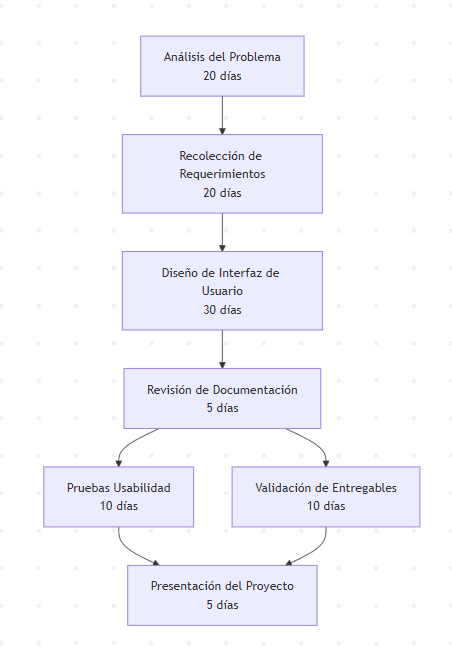
\includegraphics[width=0.60\textwidth,keepaspectratio]{./Media/Ruta Critica V3.png}%
  }
  \caption{Mapa visual de la Ruta Crítica del proyecto}
\end{figure}


%%==========================================================================================%

\clearpage
\chapter{Requerimientos y Normativas}


\section{Requerimientos Funcionales}

\begin{table}[htbp]
    \centering
    \caption{Tabla de requerimientos funcionales}
    \label{tab:requerimientos_funcionales}
    \normalsize
    \renewcommand{\arraystretch}{1.7}
    \setlength{\tabcolsep}{12pt}
    \rowcolors{2}{gray!10}{white}
    \begin{tabularx}{\linewidth}{>{\columncolor{gray!20}}m{1.5cm} >{\columncolor{white}}m{3.2cm} >{\raggedright\arraybackslash\columncolor{white}}X >{\columncolor{gray!10}}m{2.2cm}}
    \toprule
    \rowcolor{gray!40}
    \textcolor{black}{\textbf{ID}} & \textcolor{black}{\textbf{Requerimiento}} & \textcolor{black}{\textbf{Descripción}} & \textcolor{black}{\textbf{Prioridad}} \\
    \midrule
    RF-001 & Registro facial & Implementar mecanismo de reconocimiento facial para registro automático de entrada del alumnado. & \textbf{Alta} \\
    RF-002 & Herramienta docente & Proporcionar herramienta digital a docentes para verificar/registrar asistencia. & \textbf{Media} \\
    RF-003 & Consulta padres & Plataforma en línea para consulta de asistencia en tiempo real por padres. & \textbf{Media} \\
    RF-004 & Control de acceso & Restricción de acceso a personas no autorizadas con validaciones técnicas. & \textbf{Alta} \\
    RF-005 & Gestión de datos & Gestión segura de información de accesos y asistencia escolar. & \textbf{Alta} \\
    \bottomrule
    \end{tabularx}
\end{table}

\clearpage
\section{Necesidades de Usuario}

Se realizó una encuesta a estudiantes y docentes de la UPP para conocer su percepción sobre el sistema de control de acceso y la posible implementación de reconocimiento facial. Los resultados clave fueron:

\begin{itemize}
    \item El 97.6\% desea un acceso más seguro.
    \item Las opciones preferidas para un nuevo sistema son: credenciales magnéticas (51.2\%), huella digital (41.5\%) y reconocimiento facial (36.6\%).
    \item El 90.2\% estaría dispuesto a proporcionar su imagen para el acceso.
    \item Las principales preocupaciones son la seguridad de la información (53.7\%), errores del sistema (39\%), privacidad de datos (36.6\%) y la incomodidad por grabación (19.5\%).
    \item Necesidades principales: reducción de tiempos de espera (85\%), facilidad de uso (90\%), consulta en tiempo real (72\%) y seguridad y privacidad de datos (68\%).
\end{itemize}

En conclusión, existe una demanda clara por un sistema de acceso más eficiente y seguro. El reconocimiento facial es viable si se prioriza la protección de datos y se informa adecuadamente a los usuarios.

\begin{table}[H]
\centering
\caption{Resumen de Respuestas de la Encuesta}
\begin{tabular}{|p{6cm}|c|}
\hline
\rowcolor[HTML]{CFE2F3}\textbf{Necesidad Identificada} & \textbf{Porcentaje (\%)} \\
\hline
Reducción de tiempos de espera & 85 \\
Facilidad de uso & 90 \\
Consulta en tiempo real & 72 \\
Seguridad y privacidad de datos & 68 \\
\hline
\end{tabular}
\end{table}

\begin{figure}[H]
\centering
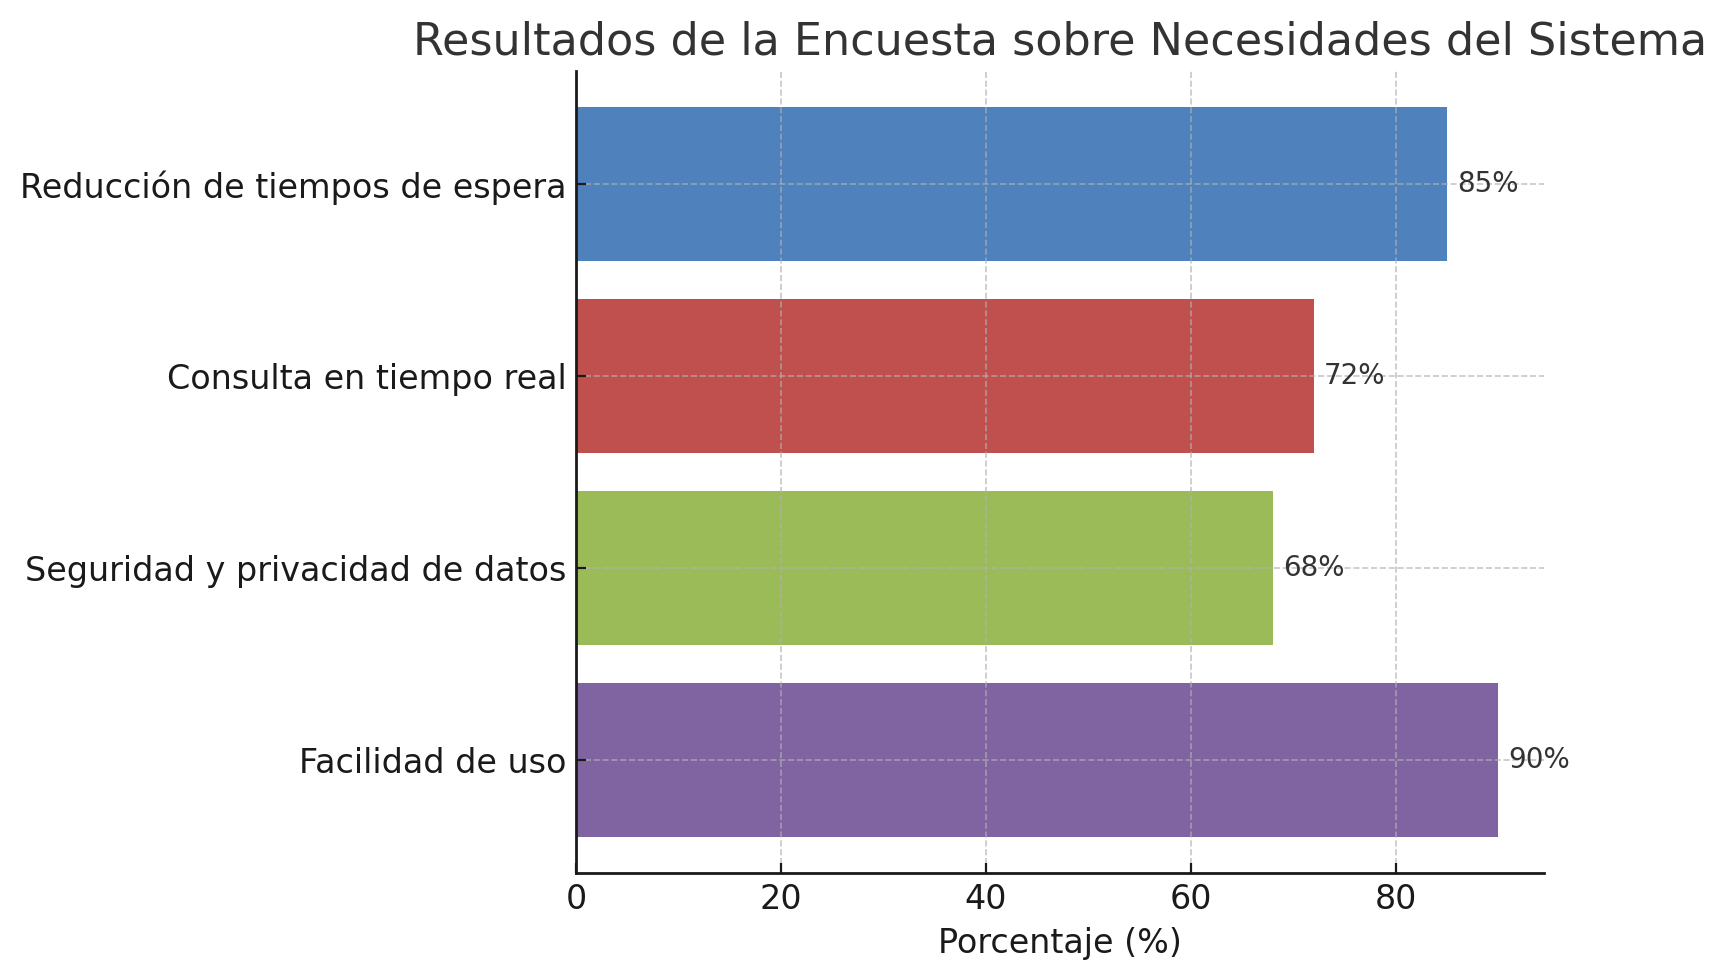
\includegraphics[width=0.8\textwidth]{./Media/grafico_encuesta.png}
\caption{Resultados de la encuesta sobre necesidades del sistema}
\end{figure}

\clearpage
\section{Normativas}

Para asegurar la calidad y seguridad en el Proyecto Argos, se adoptaron las siguientes normativas internacionales clave. Estas guían el desarrollo, la gestión y la protección de la información en el sistema:

\subsubsection*{ISO 9001:2015 – Sistemas de Gestión de la Calidad}
Establece un sistema de gestión de calidad basado en la mejora continua y la satisfacción del cliente. En Argos, se aplica para documentar procesos, auditar actividades clave y asegurar que cada entregable cumpla los requisitos funcionales y no funcionales definidos desde el inicio del proyecto.

\subsubsection*{ISO/IEC 25000 – Calidad del Producto de Software (SQuaRE)}
Proporciona criterios para evaluar la calidad del software en funcionalidad, usabilidad y eficiencia. Permite definir atributos medibles, estandarizar pruebas con usuarios finales (alumnos, docentes y padres de familia) y detectar posibles mejoras antes de la implementación final.

\subsubsection*{ISO/IEC 27001 – Seguridad de la Información}
Se enfoca en la gestión de la seguridad de la información, esencial para proteger los datos biométricos y registros de asistencia. Incluye prácticas de gestión de riesgos, uso de cifrado y autenticación segura, así como políticas de respaldo y recuperación ante incidentes.

\subsubsection*{ISO/IEC 29110 – Ingeniería de Software para PYMES y Equipos Pequeños}
Pensada para proyectos pequeños, facilita la documentación simple, la definición clara de roles y responsabilidades, y la adopción de procesos ágiles y estructurados en las fases de diseño, codificación, pruebas y validación del sistema.

\subsubsection*{Conclusión}
La integración de estas normativas fortalece la calidad y seguridad del sistema, asegurando un producto confiable, seguro y alineado con estándares internacionales. El Encargado de Calidad supervisa su aplicación y verifica, mediante auditorías internas, que cada práctica esté alineada con estos lineamientos.


%%==========================================================================================%
%
%\clearpage
%\chapter{Diseño de la UI}

\backmatter
% bibliography, glossary and index would go here.

\end{document}